\documentclass{article}
\usepackage{mathtools}
\usepackage{amssymb}
\usepackage{amsthm}
\usepackage{physics}
\usepackage{stmaryrd}
\usepackage{bbm}
\usepackage{hyperref}
\hypersetup{
    colorlinks=true,
    linkcolor=blue,
    }
\usepackage{biblatex}
\addbibresource{refs.bib}

\begin{document}

\tableofcontents

\section{Motivation}

We were given several datasets from the website ??? which sells a variety of board games. This website collects data for every article, such as reviews and grades posted by the users. 
\newline\newline
Our task was to treat and analyze this data to try to gain information from it. One purpose was to classify these reviews and being able to predict the sentiment of review (positive or negative). 

\section{Analysis on the data}

\subsection{Game score - comment}

\begin{figure}[h]
  \centering
  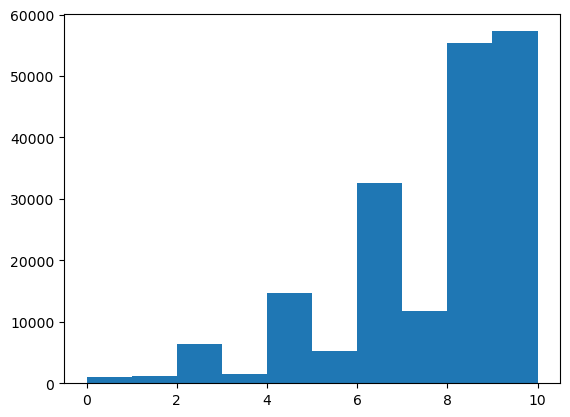
\includegraphics[height=4cm]{scores.png}
\end{figure}

\subsection{Game type - description}

\section{Corpus to vectors}

\subsection{Preprocessing}

Raw text data might contain unwanted or unimportant text due to which our results might not give efficient accuracy, and might make it hard to understand and analyze. So, proper pre-processing must be done on raw data.
\newline\newline

We had to remove punctuation, URLs, numbers, accents, stopwords.
Stopwords are commonly used words in a language that are considered to have little or no significance in determining the meaning of a text.
`not' is not a stopword, because it might indicate the opposite sentiment.
\newline\newline
We also applied Stemming that reduces words to their root forms. It minimizes the confusion around words that have similar meanings and lowers the complexity of the input space. However, it comes at the cost of throwing information away.

\subsection{One Hot Encoding}

One Hot Encoding is a vector representation of a word in vocabulary, ie the unique list of all the words appearing in the documents.
If the vocabulary size is n, each word in the vocabulary is therefore represented as a vector of size n. It takes binary values: 1 for the corresponding word and 0 otherwise.

\paragraph{On the implementation:}

We can represent the set of sentences as a tensor of shape (a, b, c) ie a matrices (number of sentences) of shape (b,c) where b represents the number of words in the sentence and c the vocabulary size.

\paragraph{Advantages:}

\begin{itemize}
  \item Intuitive and easy to implement
\end{itemize}

\paragraph{Inconvenients:}

\begin{itemize}
  \item Increase in dimensionality: a large vocabulary size implies a large number of columns, taking more memory size, which results in an increase in computational cost. + The matrix is sparse.
  \item Every vector sits in the orthogonal vector space so vectors are perpendicular to each other and are considered independent to each other, which is rarely the case.
  \item High chance of multi-collinearity due to dummy variables, which might affect the performance of the model (cf. Dummy Variable Trap)
\end{itemize}

\subsection{Bag of Words}

\subsection{tf-idf}

The BoW (Bag of Words) model assumes that the importance of a term is directly proportional to
the number of its appearance in the document, this can easily be misleading
when the most common words are `stopwords'. (But it really depends on
the algorithm that we are going to use afterwards, if we do perceptron, it wouldn't matter.)

tf-idf (term frequency - inverse document frequency) first considers
the whole of a corpus, it assumes a term too frequent in the corpus has little
information. Then it considers the importance of a term in a document
as the frequency of the term in this document times a scalar
representing its information in the corpus.

$$
\begin{aligned}
\mathrm{tfidf}(\mathrm{term}) & = \mathrm{tf}(\mathrm{term}) \times \mathrm{idf}(\mathrm{term}) \\
\mathrm{tf}(\mathrm{term}) & = \frac{\# \text { of times term appears in document }}{\# \text { of terms in document }} \\
\mathrm{idf}(\mathrm{term}) & =\ln \left(\frac{\# \text { of documents }}{\# \text { of documents in corpus with term }}\right)
\end{aligned}
$$

Other possible choices:

\begin{itemize}
  \item A term can be many (succesive) words (n-gram) (e.g. to
  take into account of negations before a word)
  \item The exact formulae can be changed while the same idea remains
\end{itemize}

\paragraph{On the implementation} Il faut éviter utiliser \verb|for|, et
utiliser les fonctions numpy à la place; on utilise les matrices sparse pour
gagner de la mémoire et parfois l'éfficacité.

\paragraph{Observations}
\begin{itemize}
  \item Curse of dimensionality
  \item Preprocessing is important
\end{itemize}

\section{Treating vectors}

\subsection{Distances}

We can use euclidean distance, or we can use the distance concerning
only the angle between 2 vectors (so the `difference of lengths' of documents
is ignored).

$$
\begin{aligned}
&\text{(cosine similarity)}S(A, B) :=
\cos (\theta)=\frac{A \cdot B}{\|A\|\|B\|}\\
&\text{(cosine distance)}D(A, B) :=1-S(A, B)
\end{aligned}
$$

We see that cosine distance is better in nlp for 1. no curse of dimensionality; 2. no
need to reduce the dimension.

\subsection{Dimensionality reduction}

\begin{itemize}
  \item PCA (not useful for us, every new word (if not a stopword) can not be ignored and their linear combinations have no meaning)
  \item t-SNE (only useful for visulization?)
\end{itemize}

After the reduction of dimensionality, we may do a visulization; but
bad visulization results don't necessarily mean bad classification result.

\subsection{Topological data analysis}

Try citation \cite{Zhu_2013}

\subsection{k nearest neighbour}

One predict the information associated with a vector by the majority
of information associated with its neighbours (within k nearest).

For comments of notes 4~7, they are more or less neutral, we can't
say if it is definitely positive or negative as human-being. So we choose
to do our algorithm on comments of extremities.

\paragraph{On the implementation} \begin{itemize}
  \item We favor the nearer information when there is a tie.
  \item Python is not a well typed language, it is so easy to have
  ridiculous bugs.
  \item cosine distance works much better than euclidean distance.
\end{itemize}

\paragraph{Positive} \begin{itemize}
  \item Easy to implement
\end{itemize}

\paragraph{Negative} \begin{itemize}
  \item Supervised
\end{itemize}

\paragraph{Testing} Given a label data set, we can test individually
for each point because of the property of the algorithm (it adapts
naturally to the data without this point), and get the expected
accuracy.

\subsection{Perceptron}

\paragraph{On the implementation}
% \begin{itemize}
% \end{itemize}

\section{Testing and evalutation of models}

\paragraph{On the implementation} \begin{itemize}
  \item Use the same seed.
  \item Balance the numbers of negatives and positives.
  \item Choose 2 extremities.
\end{itemize}

\printbibliography

\end{document}
